\section{CHESS - Lucas Weber}


\begin{frame}
	\frametitle{What is CHESS?}
	\begin{columns}
		\begin{column}{0.5\textwidth}
			\begin{itemize}
				\item \textbf{C}lassification of \textbf{H}eterogenous \textbf{S}ensor \textbf{S}ignals\footnotemark
				\item Hierarchical approach to a real-world sensor mapping problem (SIEMENS power plants)
				\item Deals with a wide variety of sensor signals and tries to map those to labels used for maintenance and monitoring
			\end{itemize}
		\end{column}
		\begin{column}{0.45\textwidth}
			\vspace*{-3em}
			\begin{flushright}
				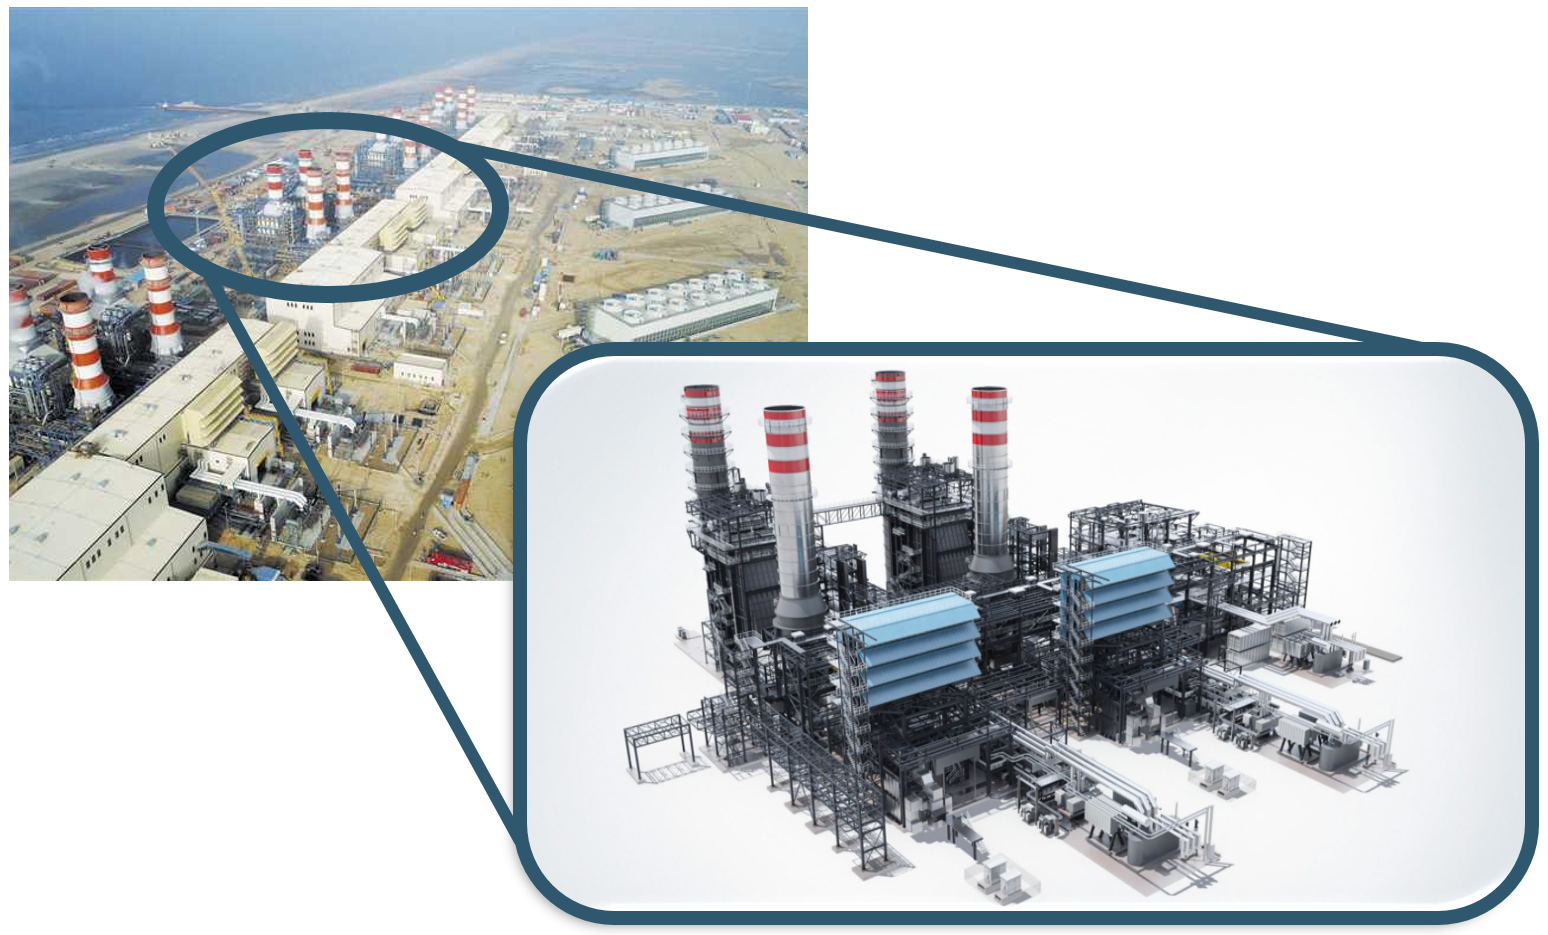
\includegraphics[width=0.8\textwidth]{img/research/PowerPlant.png}
				\begin{center}
					
\includegraphics[width=0.4\textwidth]{img/research/SElogo.png}
				\end{center}
			\end{flushright}
		\end{column}
	\end{columns}
	\footnotetext{Just recently started. Still working on the acronym and name!}
\end{frame}

\begin{frame}
	\frametitle{How could you contribute?}
	\begin{columns}
		\begin{column}{0.6\textwidth}
			\begin{itemize}
				\item We approach the high complexity problem from a hierarchical perspective
				\item The problems mostly contain time series processing, sensor fusion and pattern detection in time series
				\item We already identified the following challenges (for students or research work):
				      \begin{itemize}
					      \item Region of interest detection in power output signals
					      \item Feature engineering for sensor event response
					      \item Identification of active sensors during entity events
				      \end{itemize}
			\end{itemize}
		\end{column}
		\begin{column}{0.4\textwidth}
			\vspace*{\fill}
			\begin{flushright}
				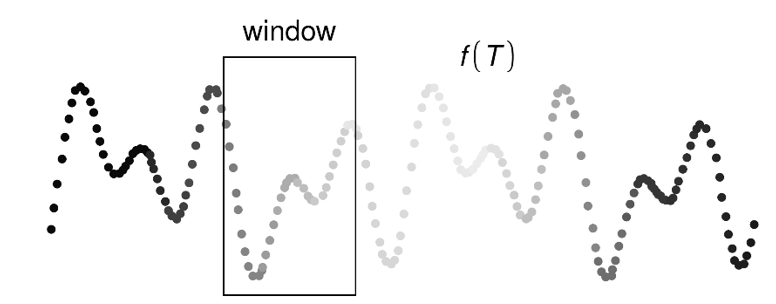
\includegraphics[width=0.8\textwidth]{img/research/ROIselection.png}
			\end{flushright}
			\vspace*{\fill}
		\end{column}
	\end{columns}
	\footnotetext{Just recently started. Still working on acronym and name!}
\end{frame}
